\section{Probabilitic Degree Anonymization}
The uncertainty injecting scheme resembles the degree anonymization method designed for the deterministic graph. One common heuristics is to select the perturbation budget for each selected edge $e=(u,v)$, depending on properties of  the vertices $u$ and $v$. The perturbation will be larger for edges that connect unique vertices, which, require higher levels of uncertainty to ``blend in the crowd", and smaller for edges that connect more ``typical" vertices. Note that, it requires one effective method to capture how typical a given vertex is among all the vertices in the uncertain graph, in terms of vertex property $P$. In this work, let us consider vertex property $P$ be node degree. In this case, namely, it is related to cluster uncertain data (distribution). The key feature of our method is to incorporate the statistical distance function for calculating the uniqueness level of vertices with regards to their node degree. 

\subsection{Uniqueness Score of Vertices}
\begin{figure*}[t!]
     \begin{subfigure}[b]{1\textwidth}
        \centering
        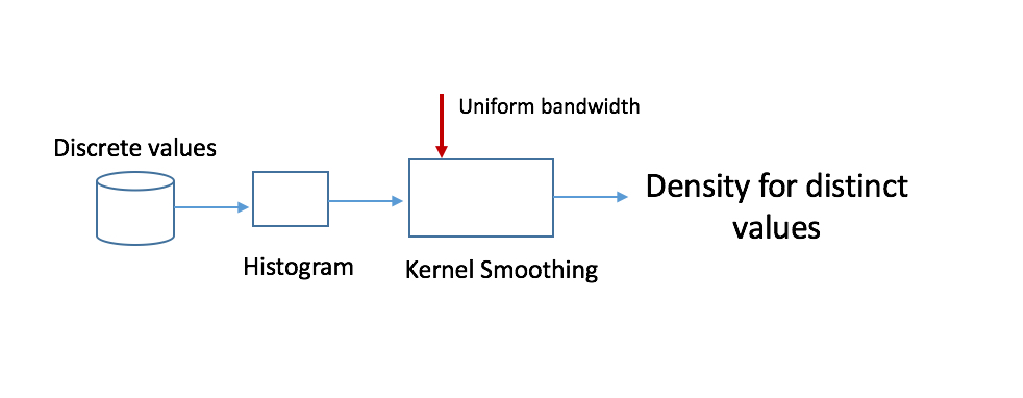
\includegraphics[scale=0.7]{figures/DegreeDistAUG/uniqueD.eps}
        \caption{Density estimation of nodes degree (Determinitic cases)}}
        \label{fig:uniqueDcal}
    \end{subfigure}%
    \begin{subfigure}[b]{1\textwidth}
		\centering
        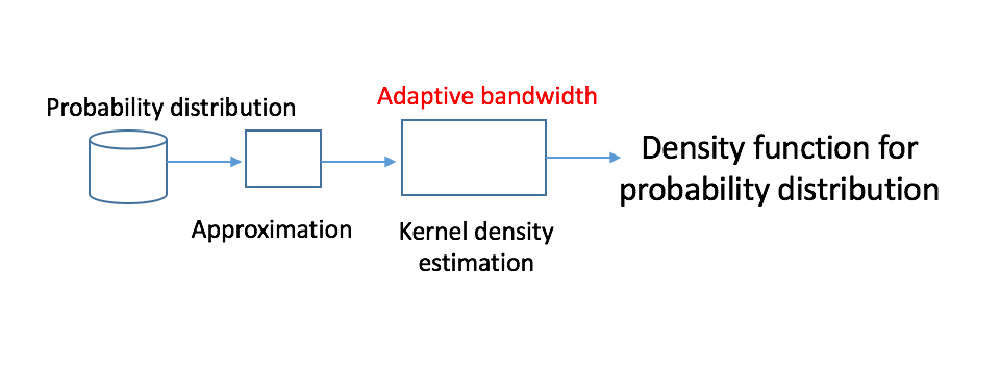
\includegraphics[scale=0.7]{figures/DegreeDistAUG/uniqueDD.eps}
        \caption{Density estimation of nodes degree (Uncertain cases)}}
        \label{fig:uniqueDDcal}
    \end{subfigure} 
    \caption{Comparison of determinitic and uncertain vertex density estimation in terms of node degree.}
\end{figure*}
For vertex properties of interest, such as degree, the majority of vertices in the real uncertain graphs are already anonymous even without random perturbation. The phenomena inherit from the one in the deterministic graph. The majority of vertices in the graph have a low degree ($\le 10$) with quite similar distribution. Hence, we aim at controlling the amount of applied perturbation, so that larger perturbation is added at vertices that are less anonymized in the original graph, namely, outlier point with respects to its degree distribution. In particular, we suggest calibrating the perturbation applied to an edge $e=(u,v) \in E_{c}$ according to the ``uniqueness" of the two vertices $u$ and $v$ with respect to the property $P$. Namely, if both $P(u)$ and $P(v)$ are in the dense region, then $r_{e}$ should be very small; on the other hand, if $P(u)$ and $P(v)$ are outlier values, then $r_{e}$ should be higher. The definition is quite similar to the ``uniqueness score", proposed in~\cite{} while extended for dealing with uncertain objects. 

Let $P$: $V \rightarrow \Omega$ be node degree defined on the set of vertices $V$ in an uncertain graph. Clearly, $\omega$ denotes uncertain object (random variable). Further, consider a distance function $d$ between  random variables in the range $\Omega$. So, for each pair of random variables,$p$ and $q$, distance $d(p,q) \ge 0$ is defined. For the degree property $P_{1}$, a natural candidate of statistical distance function is Bhattacharyya distance. For probability distribution $p$ and $q$ over the same domain $X$, the Bhattacharyya distance is defined as: 
\begin{equation*}
    D_{B}(p,q)=-ln(\sum_{x} \sqrt{p(x) \cdot q(x)})
\end{equation*}
Before the computing of statistical distance between probability distributions, we need to get the probability distribution for all the vertices in the uncertain graph. The probability distribution of $d_{v}$ may be computed exactly in time $O(n^2)$ or be approximated in time $O(n)$. The statistical distance between two probability distribution may be computed exactly in time $O(n)$. The overall complexity is $O(n^{3})$. Clearly, it is not suitable for large uncertain graphs. Note that, the uniqueness function is used for locating outlier points. For the degree property, they are nodes with high degree. In such case, we may adopt an alternative approach. Since the $d_{v}$ is the sum of independent random variable, it may be approximated by the normal distribution $N(\mu, \sigma^{2})$, where $\mu= \sum p_{e_i}$  and $\sigma^2= \sum p_{e_i} \cdot (1-p_{e_{i}})$ as implied by the Central Limit Theorem. The Central Limit Theorem becomes effective already for $n \approx 30$. For typicals size of $n$ in large uncertain graphs, the normal approximation becomes very accurate. According to the normal approximation, the Bhattacharyya distance between two normal distribution can be cacluated~\cite{} by exacting the mean and variances of two separate distribution objects: 
\begin{equation*}
    D_{B}(p,q)=\frac{1}{4} \cdot \ln{\frac{1}{4} 
                (\frac{\sigma_{p}^2}{\sigma_{q}^2} + \frac{\sigma_{q}^2}{\sigma_{p}^2}+2)}+
                \frac{1}{4} \cdot (\frac{(\mu_{p}-\mu_{q})^{2}}{\sigma_{p}^2+ \sigma_{q}^2})
\end{equation*} 
By this way, we map the object (probability distribution) from high dimension to 2D space. It speed up the computation of ``uniqueness score''. The overall time complexity is $O(n^2)$ where $n$ is the number of vertices in the uncertain graph. The quartic complexity is not suitable for dealing with large networks. 

Note that, the definition of the uniquness score is related to the kernel density estimation. For the specific method proposed in the literture~\cite{Boldi_Injecting_2012}, it adopts the gaussian function as a weighting function (kernel), the absolute difference as a distance function and the parameter $\theta$ for setting bandwidth. H
For computing the distance between probability distributions, the statistical distance functions were choosed. The remaining issue is the choice of bandwidth. Note that, the choice of bandwidth has the siginificant effect on the shape of the corresponding kernel density estimator. If the bandwidth is small, we will obtain an under smoothed estimator, with high variability. On the contrary, if the value of bandwidth $h$ is big, the resulting estimator will be over smooth and farther from the real data distribution that we are trying to estimate. Notice of the connection between uniqueness and density estimation, we adopt the adaptive bandwidth kernel density estimation method, {\ie}, we vary the w of the kernel in different regions of the sample space. By this way, we can get the statistical robust estimation of the distribution of all the vertices in the input uncertain graph in an efficient way. 
